\chapter{Available high-throughput normal human datasets}
\label{ch:datasets}

\begin{comment}
\setlength{\epigraphwidth}{0.8\textwidth}%0.57
\setlength{\epigraphrule}{0pt}%0.1
\epigraphhead[70]{%
\epigraph{Data! Data! Data! I can’t make bricks without clay!}{Sherlock Homes\\
(Sir Arthur Conan Doyle)}}
\end{comment}


In the past few years, many laboratories studied the expression
of genes within normal humans at the transcriptome and at
the proteome levels. In this chapter, I review the data I use within my thesis
and explain how it has been reprocessed.
Besides the results I report in the subsequent chapters,
the present one also provides the basis for work
I have co-authored\footfullcite{Wright-2016}.

When not stated otherwise, all the computational processing of the \Rnaseq\ part
described here have been performed by myself under the supervision of
\alvis. I also received general feedback from Dr Mar Gonzalez-Portà,
Dr Johan Rung and \nuno. The proteome data has been processed by \james.


\section{Introduction}

Every dataset with which I worked fits three main criteria.
First, they comprise normal human samples from at least three kinds of tissues.
Secondly, gene expression
quantifications are based on \Rnaseq\ for the transcriptome or on label-free \ms\
for the proteome\footnote{These
technologies are non-targeted high-throughput and
allow in theory to study the whole
repertoire of \glspl{RNA} or proteins in a sample.}.
Finally, the \emph{raw} data is available and reusable.

In the next section, I first describe the \Rnaseq\ and the \ms\ data I use
in my thesis; then I detail how these data have been processed to be
employed in the next chapters for various analyses that explore the transcriptome,
the proteome and finally, the comparison and integration of these two
biological layers.


\section{Transcriptome RNA-Seq studies}
\label{sec:rnaseq-data}

For my thesis, I had to disregard a few studies as the raw data was not fitting
the reusability point.
Indeed, many times I came across (outdated) studies with ambiguous encoding
format for the raw data.
I was also unable to get the information from the original authors.

I describe hereinafter the five transcriptomic datasets I used
in the chronological order of their first public release.
\Cref{tab:Trans5DF} summarises the main characteristics of these datasets.

\begin{sidewaystable}
           \centering
           \caption[General description of the 5 transcriptomic datasets
           (\Rnaseq) used for this study]{\label{tab:Trans5DF}\textbf{General
           description of the 5 transcriptomic datasets (\Rnaseq) used for this
           study}\\\footnotesize{Illumina Body Map (IBM) has not \enquote{regular}
           technical replicates as the \enquote{replicates} are the product of
           different protocols,\\thus are unfit to estimate the specific noise of
           either protocol (single-end or paired-end).\\
           \NB\ The protocols used for \Gtex\ and Castle datasets are not the same:
           \\\Gtex\ is following the most common ribodepletion protocol, while\\
           Castle is based on  a targeted amplification protocol.\\
           %\mynormalcheckmark\ indicates that the dataset presents the
           %characteristic, and \\(\mynormalcheckmark) that one (or more) of the
           %required criteria of the characteristic is lacking.\\
           }}
       \begin{tabular}{@{}cccccccccc@{}}
       \toprule
       \multicolumn{1}{c|}
           {\multirow{2}{*}{ArrayExpress ID}} &
            \multicolumn{1}{c|}{\multirow{2}{*}{Data ID}} &
            \multicolumn{2}{c|}{\begin{tabular}[c]{@{}c@{}}Library\\Preparation\end{tabular}} &
            \multicolumn{2}{c|}{Sequencing} &
            \multicolumn{2}{c|}{Replicates} &
            \multicolumn{1}{c|}{\multirow{2}{*}{\begin{tabular}[c]{@{}c@{}}Tissue\\
                    Number\end{tabular}}} &
            \multirow{2}{*}{\begin{tabular}[c]{@{}c@{}}Multi-sampling\\ from the \\ same
            individual\end{tabular}} \\
            \cmidrule(lr){3-8}
            \multicolumn{1}{c|}{} & \multicolumn{1}{c|}{} &
            \multicolumn{1}{c|}{\begin{tabular}[c]{@{}c@{}}Whole\\ RNA\end{tabular}} &
            \multicolumn{1}{c|}{\begin{tabular}[c]{@{}c@{}}PolyA\\ selected\end{tabular}} &
            \multicolumn{1}{c|}{\begin{tabular}[c]{@{}c@{}}Single\\ end\end{tabular}} &
            \multicolumn{1}{c|}{\begin{tabular}[c]{@{}c@{}}Paired\\ end\end{tabular}} &
            \multicolumn{1}{c|}{Biological} & \multicolumn{1}{c|}{Technical} &
            \multicolumn{1}{c|}{} &  \\
       \midrule
       E-MTAB-305 & Castle & \mycheckmark\ &  & \mycheckmark\ &  &  &  & 11 &  \\
       E-GEOD-30352 & Brawand &  & \mycheckmark\ & \mycheckmark\  &  &
           \mycheckmark\  &  & 8 &  \\
       E-MTAB-513 & IBM &  & \mycheckmark\ & \mycheckmark\ & \mycheckmark\ &  &
           (\mycheckmark) & 16 &  \\
       E-MTAB-2836 \footnotesize{(and E-MTAB-1733)}& Uhlén &  & \mycheckmark\ &
           & \mycheckmark\ & \mycheckmark\  & \mycheckmark\  & 32 &  \\
       E-MTAB-2919 & Gtex (v4)  &  & \mycheckmark\ &  & \mycheckmark\ &
           \mycheckmark\ &  & 54 & \mycheckmark\\
       \bottomrule
       \multicolumn{10}{p{.8\textwidth}}{\raggedright\
           \mynormalcheckmark\ indicates that the dataset presents the
           characteristic, and \\(\mynormalcheckmark) that one (or more) of the
           required criteria of the characteristic is lacking.}
      \end{tabular}
\end{sidewaystable}

\subsection{Castle et al.\ dataset}
\label{subsec:castlepresentation}
This dataset has been published along with the~\paper{\citetitle{castleData}}
by~\citet{castleData} who were interested in exploring the whole RNA repertoire
with sequencing-based technology. They primarily focused their study
on the non-coding part.

They used multiple-donors pooled tissues created from purchased total \gls{RNA}
samples and prepared the 11 libraries following a whole transcriptomic protocol
where nonribosomal \gls{RNA} transcripts are
amplified specifically by \gls{PCR}~\mycite{Armour:2009}.

They generated an average of 50 million sequence reads per tissue
using an Illumina Genome Analyser-II sequencer (single-end).
They trimmed their original reads to 28 \gls{nt}
and then released them through EMBL archives (\ENA{ERP000257}
and \ArrayExpress{E-MTAB-305}).

Despite several limitations (lack of replicates, old technology, small reads),
I used this dataset for two main reasons. First, it is the oldest available
\Rnaseq\ data I found that was performed on Human normal tissues. Thus, the
results congruence of this dataset to the others gives a rough assessment about
the extent of \Rnaseq\ datasets that can be integrated together in an atlas.
Secondly, as \Rnaseq\ studies are prepared mainly with polyA-selected protocols
nowadays, I was interested in gauging how the library preparation
protocols --- and the presence of \glspl{ncRNA} --- can affect the
quantifications and then the final outcomes.


\subsection{Brawand et al.\ dataset}
\label{subsec:brawandpresentation}
In the corresponding article entitled~\paper{\citetitle{VTpaper}},%
~\citet{VTpaper} focused their interest on the
evolution of the mammalian transcriptomes\footnote{While there were existing
studies on the matter, the sequencing approach was then creating new perspectives.}.

They collected 6 organs from 10 different vertebrates:
9 mammalians (including Human) and a bird. There is no technical replicate,
but there are two biological replicates per tissue:
one male and one female for every tissue but the testis (two males).
They used a polyA-selected protocol to prepare their 131 libraries (including 23
for \species{Homo sapiens}).
Hence, the samples are largely enriched in \pcgs.

They generated an average of 3.2 billion reads of 76 base pairs per sample
using an Illumina Genome Analyser IIx (single-end) and they released them
through \gls{GEO} (accession number: GSE30352).
I personally retrieved the human data from
\ArrayExpress{E-GEOD-30352}\footnote{ArrayExpress routinely imports
datasets from \gls{GEO} on a weekly basis.}.


\subsection{Illumina Body Map 2.0 (IBM)}
\label{subsec:ibmpresentation}
This dataset has been first created in 2010 and released in
2011\footnote{See:~\citetitle{ibmEnsembl} -~\cite{ibmEnsembl}} by Illumina
mostly to advertise its most recent technology improvement at that time:
the paired-end sequencing. Actually, until then, all the sequencing was done
from only one end of the \gls{DNA} or \gls{cDNA} fragments.\footnote{From that
date, most of the following transcriptome studies based on \Rnaseq\ are using
paired-end sequencing.}

The dataset comprises 16 tissues (one donor per tissue) and was prepared with a
polyA-selected preparation protocol to enrich the libraries with protein
coding genes. Indeed, Illumina main incentive to develop its paired-end
technology was to improve the accurate identification of spliced \glspl{mRNA}.

Although each sample has been sequenced twice and despite having in principle
\emph{technical} replicates, these are not ``regular'' technical replicates.
\emph{Technical} replicates, by contrast to \emph{biological} replicates,
usually imply that their processing uses the same sample source and protocols.
Thus, the error and the noise due to a specific technique could be determined.
Here, however, each tissue has been sequenced once with a single-end protocol
and once with a paired-end one to compare them together.

The sequencing was performed with an Illumina HiSeq 2000, and the reads were
released through \ArrayExpress{E-MTAB-503} (\ENA{ERP000546}), from where I
retrieved the single-end and paired-end mono-tissue samples.

I use this dataset despite the lack of biological replicates.
Indeed, for an extended time,
it was the most extensive freely available \Rnaseq\ dataset of human
tissues. Hence, it has been referenced many times in the literature
since its release.

\subsection{Uhlén et al.\ dataset}\label{subsec:uhlenPresentation}

Uhlén et al.\ have created an atlas,
\hFo{Human Protein Atlas}{http://www.proteinatlas.org/},
revolving mostly around the spatial
distribution of the proteins through the Human body. They use many approaches
and techniques which also include \Rnaseq. They first released their \Rnaseq\
data of 27 normal tissues as a part of their article~\paper{\citetitle{Uhlen2014}}%
~\mycite{Uhlen2014}. Later, they extended their dataset with new samples and 5 new
tissues. The latest version was published within~\paper{\citetitle{Uhlen2015}}%
~\mycite{Uhlen2015} in \textit{Science}.

They provide (at least two) biological replicates for each of the 32 tissues.
Except for a very small number, the tissues have both male and female donors.
There are also technical replicates for many of the tissues. The total set
comprise two hundred samples, which have been picked by pathologists based on the
screening of frozen biopsy samples.

Then they prepared the libraries following a polyA-selected protocol and
paired-end sequenced them with an Illumina HiSeq 2000 or 2500. I first started
to work with the early version of this dataset
(\ArrayExpress{E-MTAB-1733} --- 171 samples for 27 tissues),
and then I upgraded my work with the extended more recent version
(\ArrayExpress{E-MTAB-2836}).

At the time of the redaction of this thesis, this normal human dataset is the
most important one that is also freely and directly available: either regarding
the number of tissues (see \Cref{tab:Trans5DF})
or the number of samples (see \Cref{tab:Lib5DF}). Therefore, its growing
number of references is unsurprising.


\subsection{GTEx data}
\label{subsec:gtexPresentation}
The Genotype-Tissue Expression (\gls{GTEx}) project is funded by the \gls{NIH}
Common Fund and aims to establish, in its authors own words,
\textquote{a resource database and associated tissue bank for the study of the
relationship between genetic variation and gene expression
and other molecular phenotypes in multiple reference tissues}. The project was first
explained in a paper from the~\cite{GTEx2013}. It consists to quickly collect
many tissues from postmortem donors so genotype-tissue expression analyses could
be done, notably \gls{eQTL} variants studies which study the modulation
of \gls{RNA} expression in function of \glspl{SNP}. The results of the
analyses are released through the \hFo{\Gtex}{http://gtexportal.org}.

As the project is quite ambitious and the collection and sequencing of the samples
are taking time, several \enquote{\emph{freezes}} of the data have been
released\footnote{Many groups are involved in collecting, producing or processing
the data. To ease the communication and work coordination,
many time points are used to reference each a specific state (version)
of the data. Each version of the data is called a \emph{freeze}.}.
My work is
including samples up to the fourth release of the pilot phase (v4). This
release includes 54 tissue/cell types (53 normal and 1 tumoral)
collected on 551 individuals for a total of 3,276 samples.

The libraries were prepared from whole tissue \gls{RNA} extracts and then
sequenced with a \mRNA\ paired-end protocol on Illumina HiSeq 2000/2500
sequencers which produced an average of 80 million reads.

For privacy reasons, the raw data is available only through controlled access via
\dbGaP{phs000424.v4.p1} (access number specific to the version of the data I used
in my study). While getting access can take time, in principle every request for
academic research is granted.

\section{Proteome Mass Spectrometry (MS) bottom-down studies}\label{sec:ProteoData}

While the transcriptomic data were retrieved and then processed within the \EBI\
either by \nuno\ or myself, the proteomic data have been picked and
handled by \jyoti\ and \james.

Until recently, compared to the transcriptome, the proteome world
was lacking in normal human tissues expression quantification
experiments. In fact, while there were human protein maps available
(\eg\ the \hFo{Human Protein Atlas}{www.proteinatlas.org}), these
are mostly reporting the spatial expression of proteins (as they are based
on immunohistochemistry or other means of identification) than quantifying
their (non-targeted) abundance in each tissue.

In 2014, two independent groups of authors, M.-S.\ Kim et al.\
and Wilhelm et al., published (in \textit{Nature},
issue 7502) their own \textquote{\emph{draft of the human proteome}}
based on the study of tissues with \ms. These two datasets complement a previous
smaller one that was publicly released but was never the object of a publication.

Hereinafter, I present these 3 datasets that I use in my thesis.
See \Crefp{fig:pipelineProt}{A} for a short summary.

\subsection{Pandey Lab data}

The Pandey Lab~\mycite{PandeyData} created the
\hFo{Human Proteome Map}{www.humanproteomemap.org} which
they released along~\paper{\citetitle{PandeyData}} in \emph{Nature}.

For their study, they processed 30 kinds of histological normal human
tissues and cell line samples (17 adult tissues, 7 fetal tissues and 6
haematopoietic cell types). The samples were created from pooled samples of three
individuals (generally two males and one female).

Then, they prepared their libraries with a label-free method to quantify
as many proteins they could. They fractionated the samples to protein level by
\gls{SDS-PAGE} and then at peptide level after trypsin digestion by \gls{RPLC}
to create 85 experimental samples. Finally, they use state-of-art \gls{MS/MS}
protocols (with high-resolution and high accuracy \glspl{FTMS}
Thermo Scientific \orbi\ instruments).
They generated about 25 million of (\gls{HCD})
high-resolution mass spectra which account for 2,212 \gls{LC-MS/MS} profiles.

The raw spectra were retrieved from ProteomeXchange via the repository
\Pride{PXD000561}.

While their effort to generate technical high quality raw data was highly
appraised by the scientific community, their processing
(identification and quantification) methods were
criticised (see~\mycite{Ezkurdia2014-qx,Deutsch2015}).
Thus, for this thesis I only use
quantification that \james\ provided to me after reprocessing the dataset
from the raw spectra.

\subsection{Kuster data}

In their approach of the human proteome map, the Kuster Lab~\mycite{KusterData}
combined newly generated \gls{LC-MS/MS} spectrum data (about 40\% of their
complete working set) with already published data (either from their colleagues
or accessible through repositories --- for the remaining 60\%). They reprocessed
the whole collection of spectra to maximise proteome coverage
and make it available through their own repositories:
\hFo{ProteomicsDB}{https://www.proteomicsdb.org/}.

The subset of data considered in my thesis is also
known as the [protein] Human BodyMap which is the part that the Kuster lab
primary generated for their own study. They collected 48 experiments covering 36
tissues (adult and fetal) and cell lines. After \gls{LDS-PAGE} fractionation and
digestion into peptides with trypsin, they processed the samples with
\gls{LC-MS/MS} to create 1,087 profiles.  Overall, that represents about
14 million of \gls{HCD}/\gls{CID} spectra from Thermo Scientific instruments
(including an \orbi).

This specific raw data subpart was downloaded from \Proteomicsdb{PRDB000042}.

\subsection{Cutler data}

This data was generated prior to the \pandey\ and the \kuster\
data as it was released in 2011 through
\hFo{PeptideAtlas}{http://www.peptideatlas.org/}~\mycite{PeptideAtlas},
IDs: [PAe001768 --- PAe001778].

It was created by Paul Cutler at Roche Pharmaceuticals.
It comprises 10 different tissues (and one sample per tissue) that after trypsin
digestion, were analysed through Thermo Scientific \gls{LTQ}-\orbi.
In final, there are 1,618 \gls{CID} profiles which counts for 13 million of raw
\gls{CID} spectra from \gls{LTQ}-\orbi\ instrument.

While this data was never published on its own, it has been used in different
studies (\eg~\mycite{KusterData}).

The raw files were accessed and downloaded from \Proteomicsdb{PRDB000012}.


\section{Constant processing pipelines}

The authors of these five transcriptomic and three proteomic studies have,
in most cases,
released themselves the quantification of the expression values either directly
(\eg~\cite{Krupp2012}) or upon requests (\eg~\cite{PandeyData}).
Third-parties also distribute
quantification for these studies either retrieved from the original studies,
as \hFoCi{BioGPS}{http://biogps.org/}{BioGPS1} or
\hFoCi{Harmonizome}{http://amp.pharm.mssm.edu/Harmonizome}{Harmonizome},
or after reprocessing the raw data as the \egxa~\mycite{EBIgxa} does.

As mentioned before,
for many reasons and despite readily available quantifications for most of the
datasets, I only used data reprocessed from raw files by myself or \nuno\
(\gtex\ data) for the transcriptomic data and by \james\
for the proteomic data.

In fact, each study has been originally processed with different protocols,
\eg\ \gtex\ data~\mycite{GTExTranscript} and \castle\
data \mycite{Krupp2012}. While the \egxa\ reprocesses raw data through the same
methods and has nowadays quantification for most of the aforementioned
datasets\footnote{\egxa\ is still lacking the \castle.},
these were still the products of different protocols\footnote{Since
the datasets were processed with different versions of
reference (Human genome build and annotation) and tools.} when I started my work.

Intuitively, we expect that different processing protocols produce
different results.
As I started to work with \Rnaseq\ data,
I noticed many potential bias sources that impact its final expression values.
Indeed, many of these have been
reported in the literature since then; in fact,
annotation versions~\mycite{annotationDiff},
contamination~\mycite{contaminationRNAseq},
quality controls~\mycite{qualityRNAseq},
mapping and quantifications pipelines~\mycite{Fonseca2014}
have great effects on the final quantification. Lastly, normalisation
methods also greatly impact the final expression figures~\mycite{Dillies2013},%
~\mycite{normSigCancerHelp}. For all these reasons,
I decided to  reprocess all transcriptomic datasets with the same exact protocol
as the first step of my study.

Likewise, there are various tools and many parameters for each processing step
needed to quantify the proteomic data. Therefore, \james\ reprocessed
uniformly the 3 datasets from the raw spectra up to the normalisation of the
protein expression values.

\subsection{RNA-Seq raw data processing}

As presented in \Cref{sub;RNAseqworflow}, there are many steps from the raw data
files to the quantification matrices on which this thesis analyses are based.
\Cref{fig:pipelineTrans} presents a general overview of the \Rnaseq\ processing
protocol I used.

\begin{figure}
    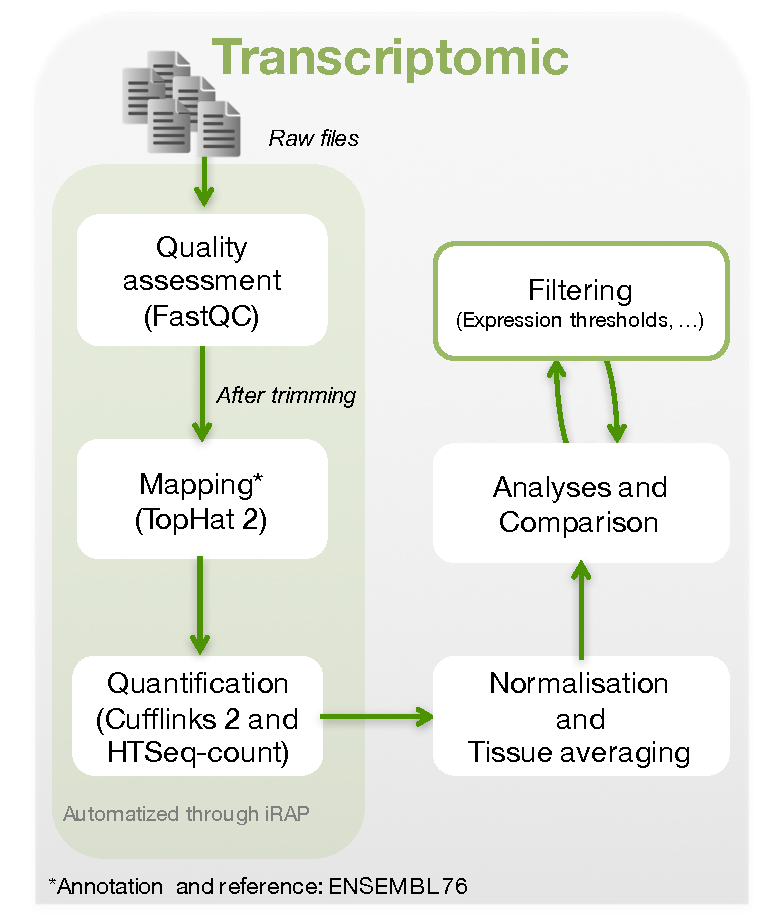
\includegraphics[scale=0.75]{datasets/pipelineTrans.pdf}\centering
    \caption[General steps for processing the transcriptomic
    data]{\label{fig:pipelineTrans}\textbf{General steps for processing the
    transcriptome.} The pipeline \irap\ integrates
    all the tools needed for the state-of-art
    processing of \Rnaseq\ data. The quality of the reads is checked and they
    are trimmed if needed. After removal of possible contaminant reads, the reads
    are aligned with \toph. The gene expression is then quantified with two
    different approaches: based on the aggregation of isomers for each gene or
    simply based on the number of aligned fragment on the gene locus defined in
    the reference. \cuffl\ provides directly \FPKM\ values. \htseq\ provides
    raw counts which were normalised by an \irap\ function into \FPKM.}
\end{figure}

I downloaded and entirely processed four of the transcriptomic datasets
myself (\castle, \vt, \ibm\ and \uhlen\ data) and
\nuno\ retrieved and processed the \gtex\ dataset (\hg{38.p1}
human genome reference and \ens{76} annotation)\footnote{As
the \Gtex\ data is involved in many project within the \EBI\
and due to its huge amount of files (number and  size --- see \Cref{tab:Lib5DF}),
it was agreed that this would be processed centrally by one person and then
redistributed to all the other interested parties. \nuno\ had this
tremendous task.}.
In this thesis,
I present results computed on the quantification of these
five datasets which have been processed through the same identical pipeline.


\begin{table}
\centering
\caption[Technical description of the 5 transcriptomic datasets]{%
\label{tab:Lib5DF}\textbf{Technical description of the 5 transcriptomic
    datasets}\\\footnotesize{I processed all the datasets but the one in
    \textit{\color{darkgray}italic}.\\
    For the Brawand dataset, I only included and processed the \species{Homo sapiens} part.}}
\begin{tabular}{@{}cccccc@{}}
\toprule
Dataset & \begin{tabular}[c]{@{}c@{}}Participant\\number\end{tabular} &
\begin{tabular}[c]{@{}c@{}}Library\\number\end{tabular} &
\begin{tabular}[c]{@{}c@{}}File\\number\end{tabular} &
\begin{tabular}[c]{@{}c@{}}Total size of\\the fastq\\raw files (GB) \end{tabular}&
    \begin{tabular}[c]{@{}c@{}}Mean number of\\biologic samples per\\tissues
    [min,max]\end{tabular} \\
\midrule
Castle        & 10    & 11    & 11    & 58    & 10 (mixture)    \\
Brawand       & 18    & 21    & 23    & 111   & 2.8  [2,3]      \\
{\small Illumina Body Map} & 16    & 36    & 48    & 1,004  & 1 \\
Uhlén         & 122   & 200   & 400   & 1,851  & 3.81    [2,11] \\
    \textit{\color{darkgray}\Gtex\ (v4)}  &
    \textit{\color{darkgray}551}  & \textit{\color{darkgray}3,276}  &
    \textit{\color{darkgray}6,552}  &
    \textit{\color{darkgray}$\sim$ 50,000}  & \textit{\color{darkgray}60.67 [4,214]}\\
\bottomrule
\end{tabular}
\end{table}

\subsubsection{Data retrieval and preparation}

I retrieved the human raw data of each dataset from \gls{ArrayExpress} and
\gls{ENA} through their identifier (see \cref{sec:rnaseq-data}). After we
received our access approval, \nuno\ retrieved \Gtex\ data from
\gls{dbGaP}.

While most of the raw files can be used as they are, an additional step is
needed for the \castle\ files. Indeed these files are using an older
\fastq\ format that is non-compliant to the most accurate and recent tools used
for this thesis.
As it is a simple matter of changing the quality score scale
(see \cref{sec:PhredScore}),
I translated these files to \gls{Phred} $33$ \fastq\ files with a
\emph{\gls{Perl}} script (see~\Cref{code:fastq}).

\subsubsection{Genome and annotation reference}

I accessed the datasets through an extended period of time. Hence, for a subset of
them, I produced many sets of results based on the \hg{37.p12}
(and later \hg{37.p13}) human reference genome and the latest available
\gls{Ensembl} annotation (73, 74 or 75) at that time.
In fact, the quality of each new annotation update is
generally greater than its predecessor\footnote{Although,
it is not unusual to have newly gene or transcript additions based on new studies
that are then removed (or fused to another) in a later version.
}.
\begin{comment}
    \TK{Ajouter example}
\end{comment}

As the \gtex\ data was processed with \hg{38.p1} and \ens{76}, that led me
to reprocess all the other four \Rnaseq\ datasets for the sake of consistency and
to avoid more biases~\mycite{h38vsh37}. Thus, unless indicated
otherwise, the results presented in the current work are
based on the \hg{38.p1} human genome reference genebuild and the \ens{76}
annotation.


\subsubsection{Data processing}

In the early stages of my research, I was processing each of the different steps
sequentially and semi-manually with the help of custom made scripts. While the
\EBI\ \gls{cluster} greatly facilitated the handling of the numerous files,
the task remained quite tedious.
Additionally,
the scripts I wrote would need a fair amount of work to achieve general
reproducibility on other platforms.

Fortunately, \nuno\ developed
an ``integrated RNA-seq analysis Pipeline'':
\hFo{\irap}{https://nunofonseca.github.io/irap/}.
This tool allows the automation of the typical
state-of-the-art and optimised workflow to study
\Rnaseq. It takes full advantages of the capacities provided by computer clusters.
Thus, I have switched to \irap\ to improve my workflow without changing any step
or parameter.

Besides the usual inputs files (raw \Rnaseq\ files and genome/annotation
references), \irap\ needs a configuration file that precisely describes the
dataset (its design and technical features) and, if needed, specific parameters
to use.
To provide full reproducibility,
each version of \irap\ is shipped with
its own set of third-party version-defined tools and default parameters.
Thus, apart of remarkably speeding up the data processing,
\irap\ also ensures the protocol integrity
across the five transcriptomic datasets I use
in my thesis regardless of who run the pipeline.

Each of the transcriptomic datasets are the products of the same version of
the \irap\ pipeline (development version 0.6.3b) and set of parameters. As the
default parameters of \irap\ are tuned for human Illumina paired-end data,
I only have to define few of them. Hence, the quality and contamination checks,
the filtering and trimming of the reads are done following the default options
of \irap.

\minisec{Quality assessment, trimming and filtering}
\irap\ uses internally
\softFo{FastX toolkit}{http://hannonlab.cshl.edu/fastx\_toolkit/} (0.0.13)
to perform the
assessment and the trimming. The recommended usual reads (see \Cref{subsub:trim})
have been discarded as were any with an overall quality score above
a threshold of 10.

As reported in the \cref{subsub:sequencing}, as the base calling progresses,
the quality of the call decreases.
On another note, some tools (mappers in particular) need
all the reads to be trimmed to the same length. \irap\ optimises the compromise
between the purity and the length of the reads to avoid more errors or
biases due to smaller reads~\mycite{Trimwisely} by trimming at most 15\% of the
original length while discarding more reads if necessary to maximise the length.

Reads that could be assigned to a likely contamination source, here
\species{Escherichia coli} (as I work with \species{Homo sapiens}),
are also discarded. A splice non-aware mapper,
\softFo{BWA}{http://bio-bwa.sourceforge.net/} (0.7.4) maps all the reads to the
contaminant genome and all the reads mapping perfectly and non ambiguously are
discarded.

\minisec{Mapping}
I mapped the reads to the genome with \irap's proposed default splice-aware mapper
\hFo{\toph}{https://ccb.jhu.edu/software/tophat/index.shtml}
(2.0.12)~\mycite{tophat2}
with its set of default predefined arguments\footnote{Indeed, \toph\ can
handle reads from many organisms by fine-tuning the parameters (\eg\ number
of mismatches or indels to tolerate), but the default parameters are adjusted
for normal human.}. Hence, I only had to provide the
genome and the transcriptome references.


\minisec{Quantification and Normalisation}
While \Rnaseq\ can be used to identify (and discover) \gls{RNA}
isoforms, I have focused my thesis on the gene level expression. Indeed, current
annotations and knowledge are still lacking in the reasons and
external conditions that impact the expression of a specific isoform over the
others. In addition, criticisms have been raised on the accuracy of distinction
between them~\mycite{tamaraRNA,ernestRNA}. Normalising gene expression
presents additional challenges than specific transcript expression,
as the definition of the gene length may be different from one lab to another.

In the framework of this thesis,
when I have to use a gene length for a computation,
I use the identical gene length definition as found in
\irap\ and \egxa.
Thus, as shown on \Cref{fig:Genelength-collapsedExons} the gene
length is defined as the sum of the length of all its \emph{collapsed} exons.

\begin{figure}
    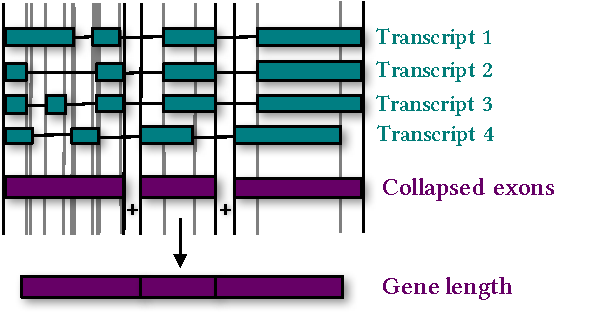
\includegraphics[scale=0.8]{datasets/collapsedExonsLinLib.pdf}\centering
        \caption[Gene length equals to the sum of the length of all its collapsed
        exons]{\label{fig:Genelength-collapsedExons}\textbf{Gene length equals to
        the sum of the length of all its collapsed exons.} This method lacks
        complete accuracy however, it provides a sufficient estimation of the
        gene length for an efficient normalisation regarding the length bias.
        The coordinates for the 5' and 3' ends of each exon is extracted from
        the annotation and they are collapsed together. This \emph{gene length}
        is unaffected by incorrect attribution of a fragment to a
        specific transcript when there are many possible options.}
    \end{figure}

As mentioned in \Cref{subsub:norm}, I used two different popular tools based on
different strategies to estimate
gene expression levels:
\hFo{\cuffl}{http://cole-trapnell-lab.github.io/cufflinks/manual/}
(2.2.1)~\mycite{cufflinks}
and \hFo{\htseq}{http://www-huber.embl.de/HTSeq/doc/index.html\#}
(0.6.1p1)~\mycite{htseq} (with the \texttt{intersection non-empty} mode).
These tools are also integrated in \irap.

For \cuffl, I used the mode where the multi-mapped reads are probabilistically
assigned depending on the coverage of each mapped locus. In addition,
\cuffl\ provides normalised gene expression levels by aggregating their
corresponding normalised isoform expression levels. \cuffl\ uses the
\cref{eq:rpkm-fx} to normalise isoform expression levels. The length of the
isoforms are extracted from the reference.

On the other hand, \htseq\ provides only \emph{raw} counts for the feature of
interest. \irap\ provides an internal \FPKM\ normalisation function that
is an implementation of the \cref{eq:rpkm-fx}. As I requested \htseq\ to work at
gene level, this formula requires gene lengths which are computed with the
aforementioned method.

All the configuration files I created for this thesis may be found at
\addressToirapConfFiles.

\subsection{MS shotgun data processing}

After retrieval of the data from \gls{Pride} and \gls{Proteomicsdb},
\james\ reprocessed the three proteome \ms-based datasets.
\Cref{fig:pipelineProt} illustrates the pipeline that processed the three
datasets in a consistent and optimal manner. I summarise this protocol
in \Crefp{fig:pipelineProt}{}
and in the following \cref{subsub:spectralProcessing,subsub:seqDBseeking,%
subsub:spectralIDDBsearch,subsub:resultsFiltering}.
See~\mycite{Wright-2016,Weisser2016-pipeline} for more details.

  \begin{sidewaysfigure}
      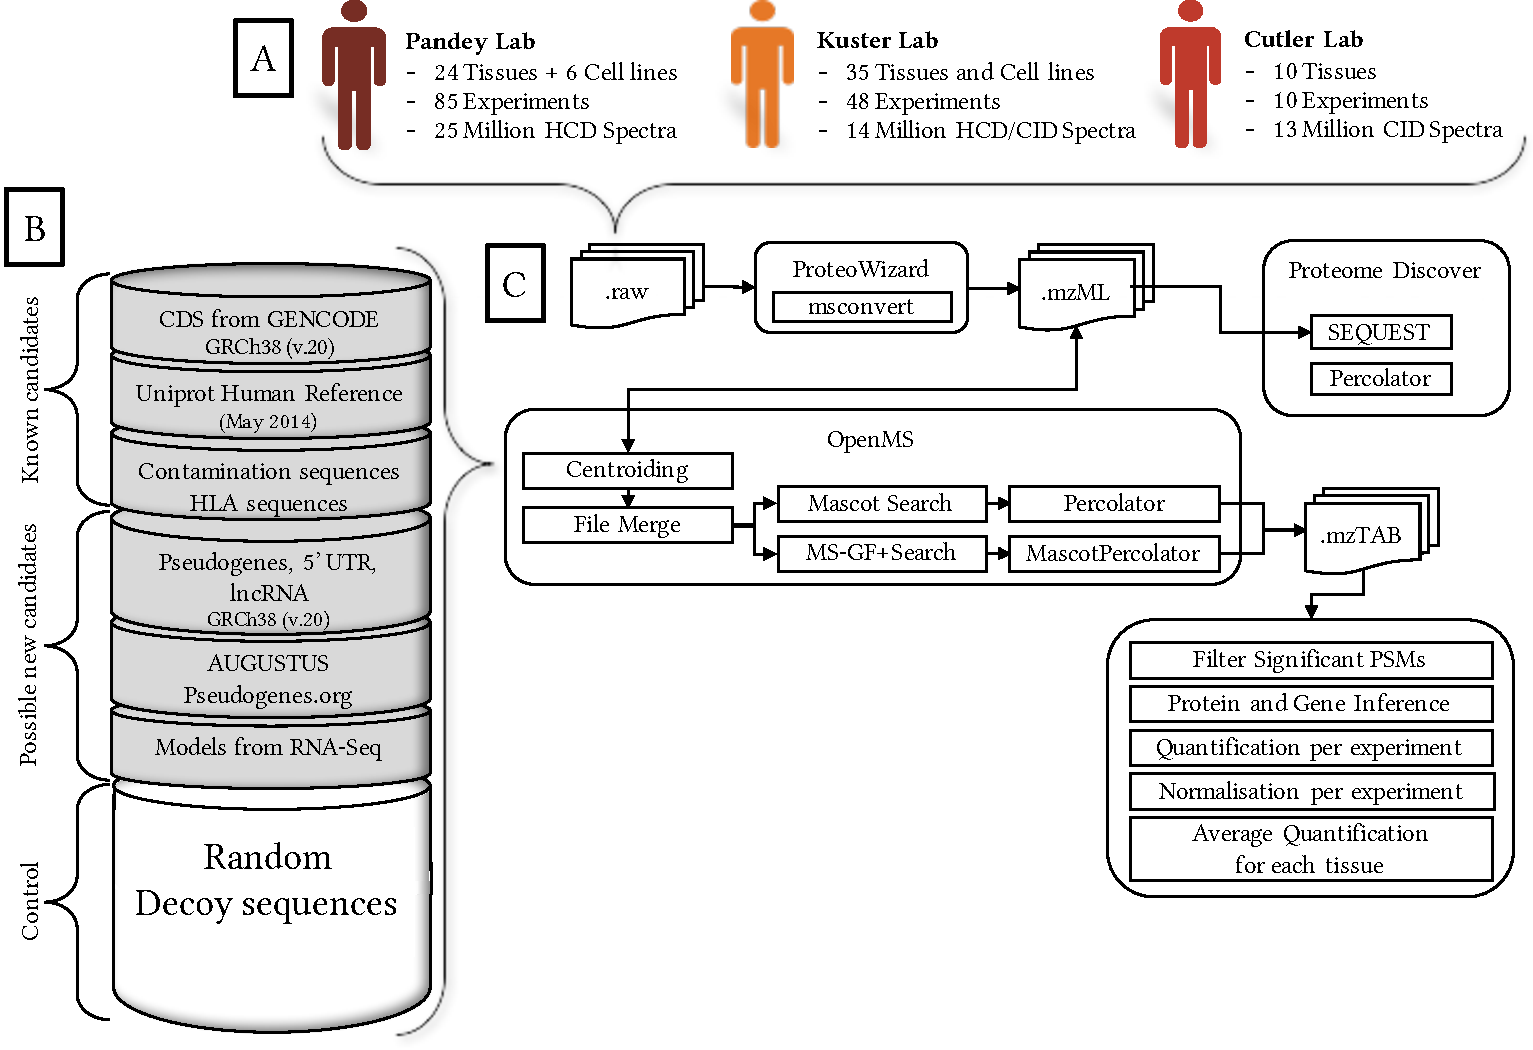
\includegraphics[scale=0.75]{datasets/pipelineMS-2.pdf}\centering
      \caption[General steps for processing the proteome
      data]{\label{fig:pipelineProt}\textbf{General steps for processing the
      proteome.} [Adaptation of courtesy materials from \james].\\
      (\textbf{A}) The 3 datasets have been processed through the
      same pipeline. I only use their normal tissues samples and I also discard
      the cell lines. (\textbf{B}) Extensive sources of protein sequences were
      used for the search database, including prediction of novel proteins.
      Contamination and decoy sequences were also included to allow for \gls{FDR}
      estimation. (\textbf{C}) State of the art workflow was used to process the
      \ms\ data from raw files.
      This workflow combines multiple \ms\ search engines and
      post-search evaluation tools. Results were filtered by peptide length,
      \gls{FDR}, \gls{PEP} and agreement between the multiple search algorithms.
      \\\NB\ There is no relation between the real size of
      the database parts and their representation.}
  \end{sidewaysfigure}

\subsubsection{Spectral processing}\label{subsub:spectralProcessing}

The \soft{msconvert} module of \softFull{ProteoWizard}%
{http://proteowizard.sourceforge.net/}{ProteomeWizard}{v3.0.6485}
converted all the files to the standard format mzML.\@
\softCi{TOPP}{Topp} from
\softFull{OpenMS}{http://www.openms.de/}{openMS2016}{pre-v2.0 development build},
processed the raw spectra. Notably, \soft{PeakPickerHiRes} to centroid them
and \soft{FileMerger} to merge the ones from the same fractionated experiments.

\subsubsection{Sequence database creation and preparation for searching}%
\label{subsub:seqDBseeking}

The target sequence database is a critical element of the \ms\ pipeline and thus,
\james\ has carefully designed it.
It combines six different parts, three based on
known protein sequences and three other covering possible new protein candidates.

The known sources include the complete human \hg{38} (v.20) \gls{CDS} translated
sequences from \gls{GENCODE}; the human reference proteome from
\gls{Uniprot}\footnote{%
\gls{Uniprot} --- \Href{http://www.uniprot.org/}}~\mycite{UniProt2017}
(in its May 2014 version); common contamination protein
sequences\footnote{Contamination sequences ---
\Href{http://maxquant.org/contaminants.zip}}
and \gls{HLA} sequences\footnote{\gls{HLA} sequences ---
\Href{http://www.ebi.ac.uk/ipd/imgt/hla/download.html}}.

The sources for potential
novel proteins included a selection of non-coding gene sequences (including
pseudogenes, \gls{lncRNA} and untranslated regions) from \gls{GENCODE}
\hg{38} (v.20); prediction of novel sequences with
\softFoCi{\mbox{AUGUSTUS}}{http://bioinf.uni-greifswald.de/augustus/}{Stanke2004};
a set of two-consensus predictions (December 2013)
from \softFoCi{Pseudogene.org}{http://pseudogene.org/}{pseudogenesOrg}
and three-frame translated \Rnaseq\ transcript sequences.
These translated sequences include models
built on \ibm\ by \gls{Ensembl} and by the Kellis lab in addition with
models built on different \gls{ENCODE} cell lines by Caltech and CSHL\@.
Precautions were taken with the handling of the overlapping regions
and with the sequence three-frame translations.

\softFo{Mimic}{https://github.com/percolator/mimic} generated the randomised
decoy sequences (equal sizes of the target database sequences).
The different databases were then merged together.
It is represented on \Cref{fig:pipelineProt}{\footnotesize B}

To account for the isobaric peptides, all isoleucine (I) residues were
converted to leucine (L) before the search and then after the search all leucine
(L) residues were converted to (J) to avoid later misconceptions.
In summary, the know coding portion of the tryptic peptides sequences represents
787,587 peptides and the novel portion provides an additional 4,211,835 peptides.

\NB\ For each peptide sequence, there is a unique identifier,
an associated source database
and when available the corresponding gene locus.

\subsubsection{Spectral identification and database search pipeline}%
\label{subsub:spectralIDDBsearch}

\Cref{fig:pipelineProt}{\footnotesize C} describes the overall workflow used by
\james\ to quantify the protein abundance in each tissue. As mentioned in
\Cref{seg:moreAlgoisbetter}, workflows involving several algorithms produce
better results. \soft{Mascot} Server~(v~2.4--- Matrix Science)~cluster produced
a first search on the mzML files submitted through \soft{MascotAdapterOnline}
(part of \soft{TOPP}). In parallel, \james\ also used  \soft{MS-GF~$+$~Search},
which involves the run of \soft{MS-GF~$+$}~(v. 10089)~\mycite{Kim2014-nj}.
\soft{MascotPercolator}~(v~2.08)~\mycite{Brosch2009-xq,Wright2012-od}
optimised and rescored the results from \soft{Mascot} and
\soft{msgf2pin/Percolator} (v~2.08\textminus1)~\mycite{Granholm2014-cw} optimised
the results from \soft{MS-GF~$+$}.
Finally, \soft{SEQUEST}~\mycite{Eng1994-eq} and
\soft{Percolator}~\mycite{Spivak2009-zd} performed a research in a
\soft{Proteome Discoverer}~(v 1.4 --- Thermo Scientific) workflow.

The different workflows used common stringent parameters for all the database
searches:
the precursor tolerance was set to 10 \gls{ppm};
fragment tolerance for \gls{HCD} spectra to $0.02$ \gls{Da} and
to $0.5$ \gls{Da} for \gls{CID} spectra;
the allowed missed cleavages limit to $3$; several amino acid modifications were
also used for the research (see~\mycite{Wright-2016}).

The research results were converted into mzTab formatted files and uploaded along
with the mzML spectra and FASTA search database to \gls{Pride}
under accession \Pride{PXD002967}.

\subsubsection{Results processing and filtering}\label{subsub:resultsFiltering}

Custom Perl scripts parsed, merged and filtered the results of each search engine
so that every \gls{PSM} had the same identification in at least two of the three
search engines.
In each case, the least confident \gls{PEP} (\ie\ the highest) was retained.

The \glspl{PSM} were then filtered to only keep matches to the three following
criteria:
\gls{q-value} equals to $0.01$ (\ie\ 1\% \gls{FDR}) at the greatest; % $\leq 0.01$
a \gls{PEP} inferior or equal to 0.05 at the greatest and
a peptide length superior or equal to 7 amino acids.
\glspl{PSM} matching contaminant or decoy sequences were also removed.

The resulting list of peptides was then used to infer the proteins with
a simple approach.
Protein clusters are created based on common matching non-null set of peptides,
\ie\ each protein cluster has at least one unique peptide.
Then, the \gls{GENCODE} \gls{CDS} and \gls{Uniprot} accession were mapped back to
\gls{Ensembl} identifiers.
The genes that were matching at least 3 unique peptides were kept for the
remaining of the analysis while the others were discarded. Protein clusters
matching several gene identifiers or failing the \emph{unique peptide} rule were
discarded. (\NB\ The list of the discarded clusters is different for each of the
proteome dataset.)

The quantification (and normalisation) of the kept proteins were computed
with the Top3~(\gls{IBAQ}) approach for each experiment.
When there were more than one experiment per tissue, the final quantification
values are the average across all the experiment of each tissue.

Compared to the original \pandey\ study, less proteins were quantified, but
the results are congruent to other previous studies on the range of detection
and quantification of \gls{LC-MS/MS}. The quantification were released along
our paper~\mycite{Wright-2016} and the reanalysis of the \pandey\ data was
also released through \egxa\ under the accession: E\textminus{}PROT\textminus{}1.

\section{Discussion}

In this chapter, I introduced the 5 transcriptomic and 3 proteomic normal
human tissues datasets on which I based my thesis.
I described how both the transcriptomic and the proteomic datasets have been
reprocessed from raw files with state-of-the-art unified pipelines
which are also using the same genome built and annotation references in the
final processed version.

As a matter of fact, I accessed the datasets through an extended period of time.
For a subset of the transcriptomic datasets,
I thus produced many sets of results with
the previous human reference genome~(\hg{37}) and
three different \gls{Ensembl} annotations (73, 74 and 75).
If the results may vary for individual genes,
the overall outcomes are congruent together hence
supporting the robustness of the findings presented in this thesis.
In addition, the products of these pipelines are in agreement with the original
studies findings --- apart for~\mycite{PandeyData}.

While we are in the era of \emph{data deluge} and \emph{big data},
the number of tissue overlaps for independent normal human studies is surprisingly small.
Most of these datasets have been (and will be) referenced through
many papers for comparison (or as control) purposes;
hence, it is essential to assess the soundness of these practices by assessing
the consistency between these datasets.

